\section{El mercado de los videojuegos}

\subsection{Industria mundial del Videojuego}
El mercado del videojuego es actualmente la industria de ocio y entretenimiento más grande, superando en tamaño tanto a la industria cinematográfica como a la discográfica. Se trata de una industria creciente, con una tasa del crecimiento del 6,6\% y que cuenta ya con más de 2.200 millones de jugadores en todo el mundo. Se espera que, en el año 2020, la cotización anual alcance los 143.500 millones de dólares \cite{libro_blanco}.

\begin{figure}[h]
    \centering
    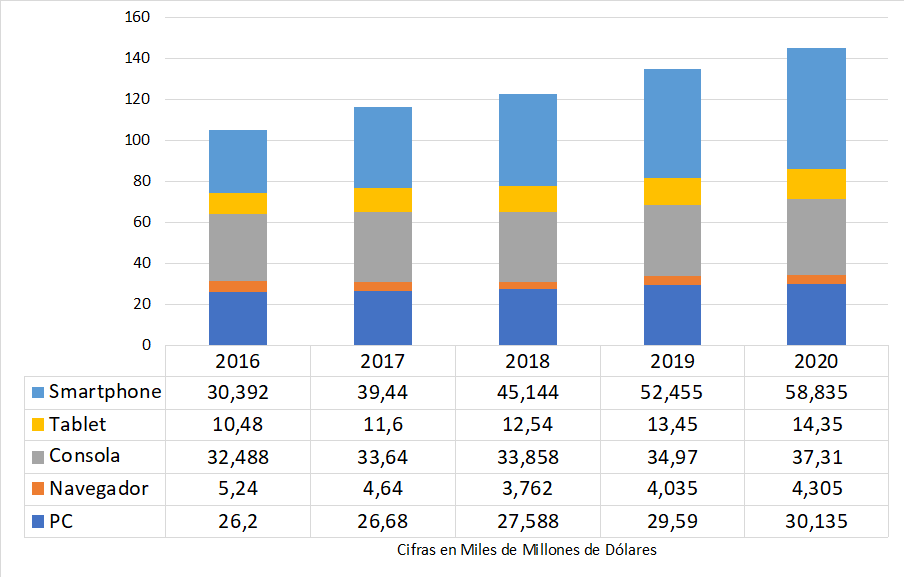
\includegraphics[width=0.8\textwidth]{images/estadodelarte/mercado/crecimiento_mercado_plataforma}
    \caption{Crecimiento Mundial de la industria del videojuego (por plataformas).}
\end{figure}

Actualmente, la plataforma de distribución que ocupa un segmento mayor del mercado son los dispositivos móviles. Debido al constante incremento de potencia de los Smarthphones, así como a su ubicuidad en la sociedad actual, el mercado de videojuegos para estas plataformas ha experimentado un incremento constante en los últimos años, superando al mercado para PC y al mercado para Videoconsolas de sobremesa. A fecha de 2017, el mercado Smarthphones ha alcanzado los 39.440 millones de dólares, lo que representa el 34\% del mercado. Por otro lado, el mercado de las consolas portátiles y el de los juegos Web casuales son los que presentan un declive más pronunciado, debido seguramente a que ocupan un nicho de mercado similar al de los juegos móviles\cite{libro_blanco}.

\begin{figure}[h]
    \centering
    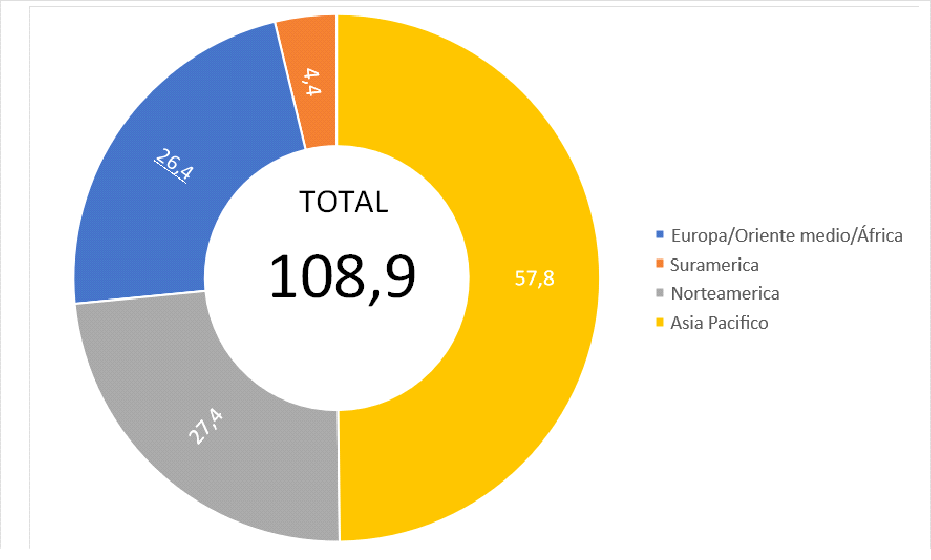
\includegraphics[width=0.8\textwidth]{images/estadodelarte/mercado/distribucion-mercado-mundial}
    \caption{Distribución por regiones del mercado del videojuego.}
\end{figure}

Si dividimos el mercado en las distintas regiones geográficas, podemos observar que Asia Pacifico lidera el mercado con un beneficio de 51.200 millones de dólares en el año 2017, un 47\% del total de los ingresos globales, de los cuales más de la mitad son generados por China, con 227.500 millones de dólares. En segunda posición se encuentra el mercado norteamericano, con 23.500 millones de dólares en 2016, representado prácticamente en su totalidad por Estados Unidos. En el ranking de los 10 mercados con mayores ingresos podemos encontrar cinco países europeos: Alemania, Reino Unido, Francia, España e Italia. Sin embargo, la diferencia en tamaño con respecto a los tres primeros mercados de la lista (China, Estados Unidos y Japón) es abismal\cite{libro_blanco}.

\begin{figure}[h]
    \centering
    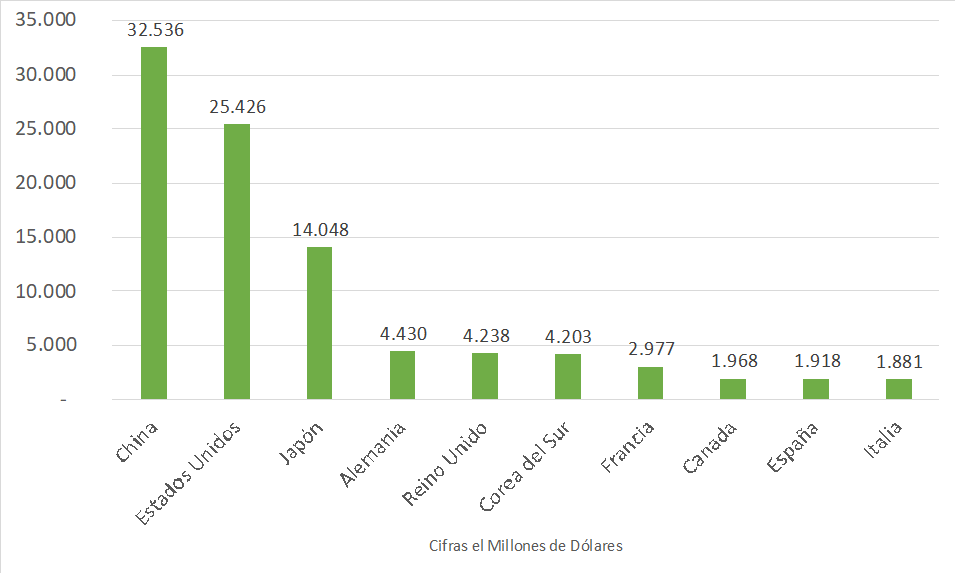
\includegraphics[width=0.8\textwidth]{images/estadodelarte/mercado/10-mayores-mercados}
    \caption{Diez principales mercados del videojuego.}
\end{figure}

\subsection{La industria de los videojuegos en España}
La industria del videojuego española es la cuarta mayor de Europa (por detrás de Alemania, Reino Unido y Francia) y la novena mayor a nivel mundial. A fecha de 2017, el mercado español del videojuego facturó un total de 1.900 millones de dolares, con un crecimiento del 20\% con respecto al año anterior. Más de la mitad de estos ingresos provienen de la venta de videojuegos españoles al extranjero, gracias a la casi total falta de fronteras para la distribución internacional de productos. Este enfoque en el mercado internacional se ve reflejado en factores como la mayor frecuencia del inglés en las producciones españolas que el propio español (99\% contra 95\%)\cite{libro_blanco}.

\begin{figure}[h]
    \centering
    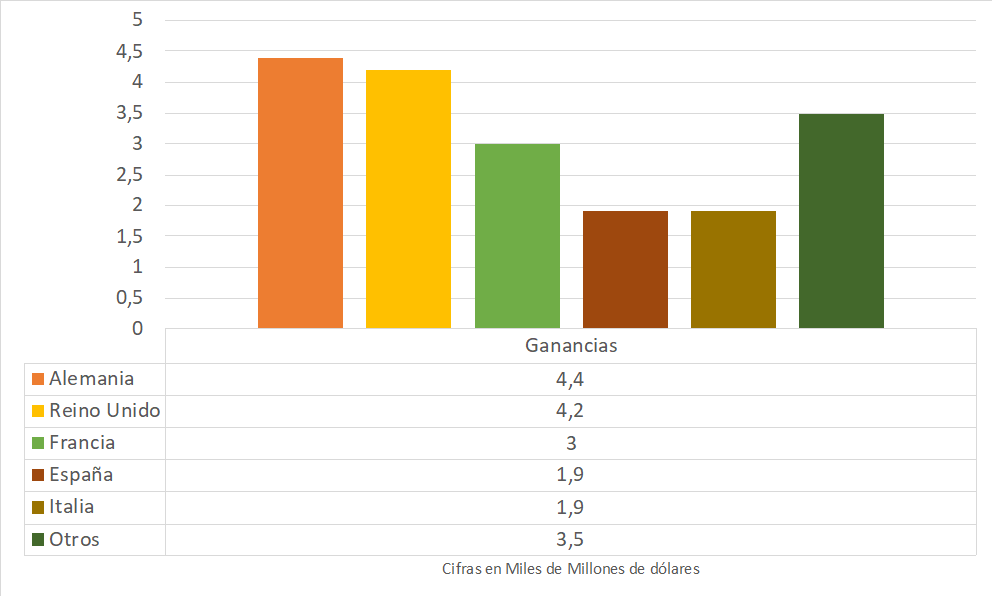
\includegraphics[width=0.8\textwidth]{images/estadodelarte/mercado/distribucion-mercado-europa}
    \caption{Mercado del Videojuego en Europa.}
\end{figure}

En total, el sector cuenta con 480 empresas en activo, a las que debemos añadir las 130 iniciativas y proyectos empresariales, que se encuentran a la espera de consolidarse como empresas en el corto o medio plazo. La mayor parte de estas empresas tienen una plantilla de menos de 5 empleados, formando el 47\% de la industria. Esto se debe en parte a la adecuación de las pequeñas empresas a la creación de juegos de pequeña escala para dispositivos móviles (el principal mercado), pero también se debe a una escasez de puestos de trabajo en las empresas de tamaño mediano y grande y a la saturación del mercado que dificulta el crecimiento de las empresas\cite{libro_blanco}.

\begin{figure}[h]
    \centering
    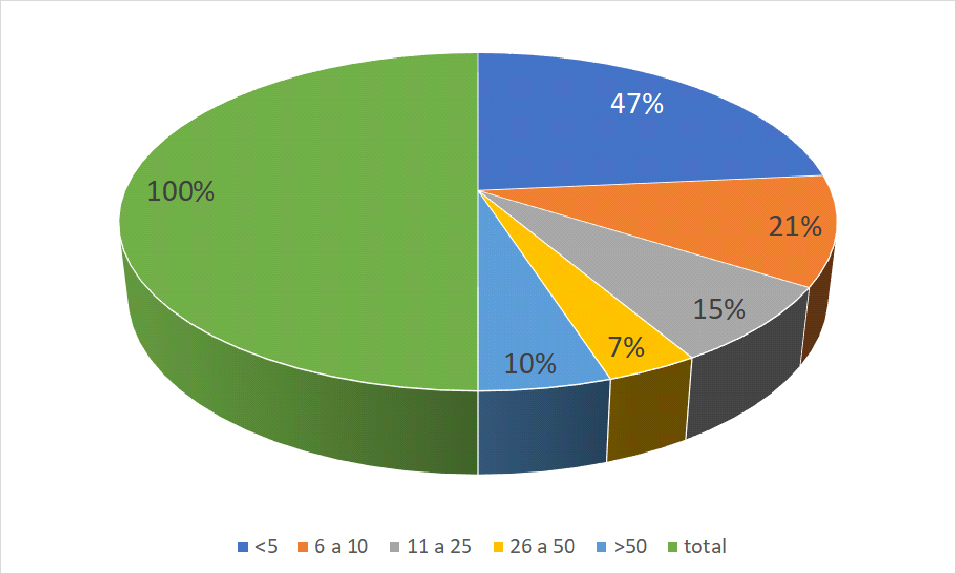
\includegraphics[width=0.8\textwidth]{images/estadodelarte/mercado/distribucion-tamano-esp}
    \caption{Distribución de las empresas en España por número de empleados.}
\end{figure}

La actividad empresarial del país se encuentra centrada en dos comunidades autónomas: Cataluña y la comunidad de Madrid. De estos dos centros principales destaca Cataluña, donde se concentra el 52\% de la facturación del país. Detrás de las dos comunidades principales se encuentran la Comunidad Valenciana, el País Vasco y Andalucía, las cuales suman entre las tres un 28\% de las empresas. El resto de comunidades se quedan muy por detrás de estas cinco primeras\cite{libro_blanco}.

\begin{figure}[h]
    \centering
    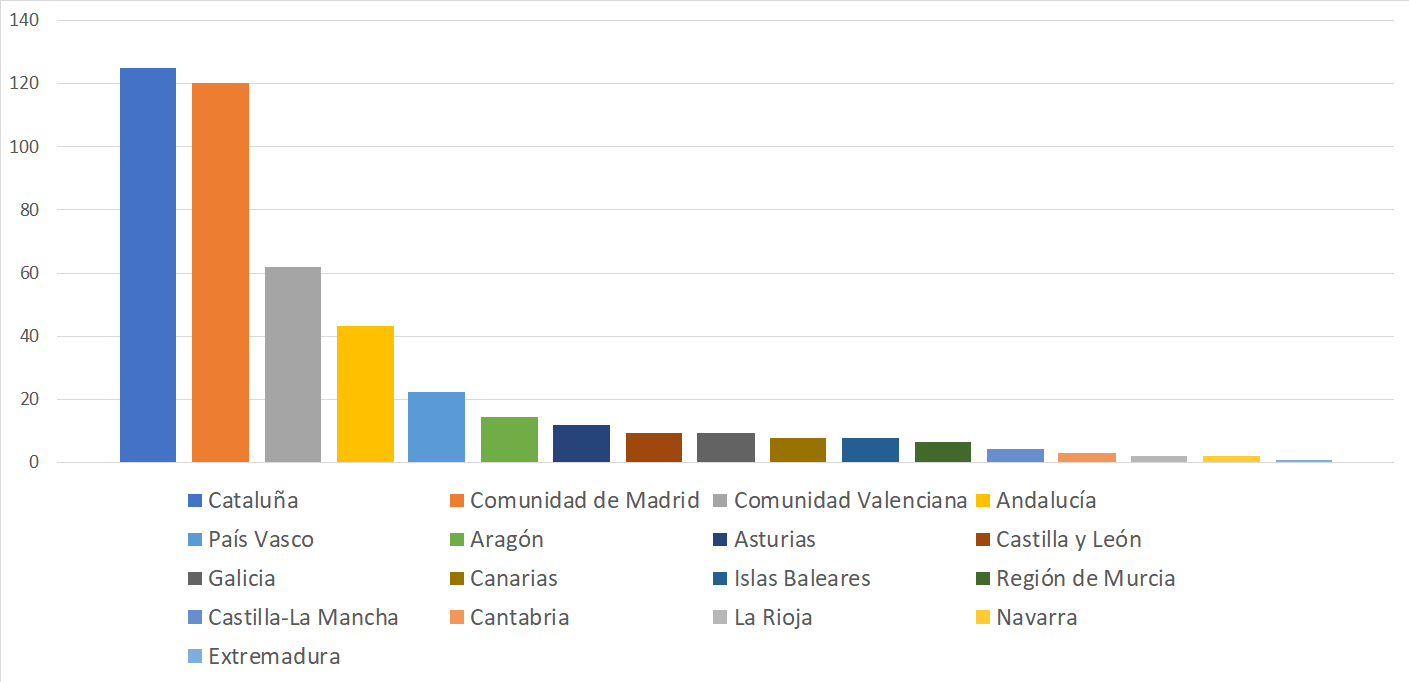
\includegraphics[width=0.8\textwidth]{images/estadodelarte/mercado/distribucion-comunidades-esp}
    \caption{Distribución de las empresas en España por número de empleados.}
\end{figure}

\subsection{Retos y tendencias actuales}
El videojuego ha sido y es una industria muy cambiante, que siempre ha intentado integrar las tecnologías más punteras, desde innovadores algoritmos de renderizado gráfico hasta exóticos dispositivos de interacción persona-ordenador.

A continuación, listaremos algunas de las tendencias que van a influir fuertemente en el mercado en los años venideros:

\subsubsection{eSports}
Los eSports, también llamados ``deportes electrónicos'', es el nombre por el cual se conocen las competiciones de videojuegos multijugador. En los eSports, los jugadores profesionales compiten entre ellos en diferentes categorías: disparos en primera persona, lucha, estrategia en tiempo real, MOBAs (Multiplayer Online Battle Arena)... La popularidad de este fenómeno ha llegado al punto en el que los principales torneos se celebran en grandes estadios, están retransmitidos en streaming por Internet e incluso están dotados con premios de grandes cantidades de dinero y que en ocasiones superan el millón de euros. Se trata de unos eventos de gran popularidad que cuentan enormes con perspectivas de crecimiento (a una tasa anual del 34\%). Esto ha provocado que se haya posicionado como un fenómeno de ocio estratégico\cite{libro_blanco}.

\begin{figure}[h]
    \centering
    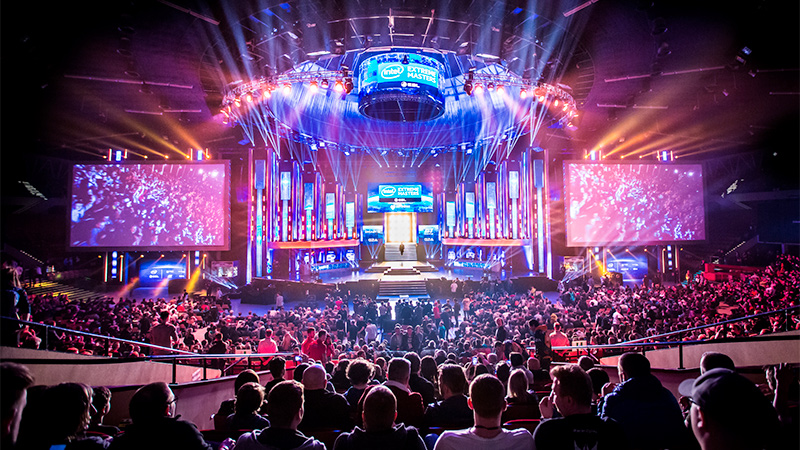
\includegraphics[width=0.8\textwidth]{images/estadodelarte/mercado/foto-torneo-esport}
    \caption{Fotografía del torneo Intel® Extreme Masters en Katowice, Polonia}
\end{figure}

El mercado de los eSports, generó en 2017 600 millones de dólares de ingresos, creciendo del 67\% con respecto al año anterior. Si la situación se mantiene, se espera que la cifra supere los mil millones de dólares en el año 2019, manteniendo un crecimiento anual superior al 34\%. En 2016, hubo 385,5 millones de personas que vieron partidos de competiciones de diversos deportes electrónicos, de los cuales 115 millones pueden ser clasificados como ``entusiastas'', es decir, espectadores regulares y participantes no muy distintos de los que encontraríamos en los deportes convencionales\cite{libro_blanco}.

\begin{figure}[h]
    \centering
    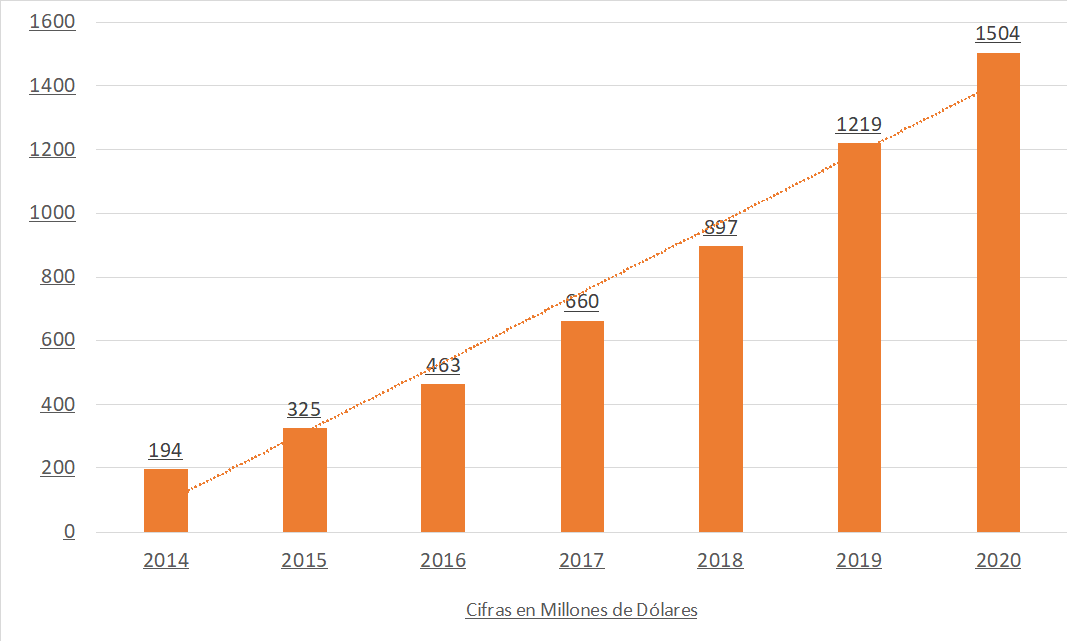
\includegraphics[width=0.8\textwidth]{images/estadodelarte/mercado/crecimiento-esport}
    \caption{Crecimiento del mercado del eSport}
\end{figure}

Existen en España diferentes empresas que en la actualidad apuestan por el desarrollo de productos que aspiran a convertirse en eSports, es el caso de Digital Legends\footnote{http://www.digital-legends.com/}, Mercury Steam\footnote{https://www.mercurysteam.com/}, PixelCream Studio\footnote{http://pixelcreamstudio.com/}, Mechanical Boss\footnote{http://www.mechanicalboss.com/}, entre otros. Sin embargo, en la mayoría de las ocasiones un videojuego online se convierte en eSports de manera orgánica, basada en el reconocimiento que la comunidad online de jugadores activos de ese videojuego le otorga. Existen eso si casos en las que una gran marca apuesta porque su producto se convierta en un eSports, realizando grandes inversiones en infraestructura, personal dedicado a la comunidad, servidores escalables para una gran masa de jugadores, premios para los torneos, entre otras muchas. 

Sin embargo, esta inversión no siempre esto asegura que su producto se convierta en un éxito. Para que un videojuego pueda convertirse en un eSport necesita contar con características básicas: tener un fuerte factor de competición, partidas cortas de no más de 1 hora, sin progresión in-game (la progresión debe basarse en las habilidades del jugador) atractivo sistema de espectador y tener un enfoque al 100\% internacional.

Pese a su gran dificultad, conseguir posicionar un producto como eSports, aporta una serie de beneficios y posibilidades: 
\begin{itemize}
\item Crear una base de fans, una comunidad, algo que aporta un núcleo de consumidores fieles al producto y que le da una nueva dimensión social, muy atractiva para muchos de los consumidores de videojuegos.
\item Prolongar la vida del producto; al ser competitivo, el jugador fija sus metas ante los otros jugadores, esto incentiva al usuario y le proporciona una motivación para seguir consumiendo.
\item Proporcionar mayor visibilidad, ya que a pesar de que los productos asentados son extremadamente sólidos, su numero es muy reducido, por lo cual hay una demanda latente de usuarios que buscan nuevos eSports.
\item Aumentar la fidelidad de los usuarios al tratarse de un mercado donde los usuarios tienen un índice de fidelidad mucho más alto que en otros.
\item Los jugadores, al estar involucrado con un producto competitivo, ven streaming, leen noticias, siguen torneos, participan en foros, lo que disminuye el riesgo de abandono del producto.
\end{itemize}

\begin{figure}[h]
    \centering
    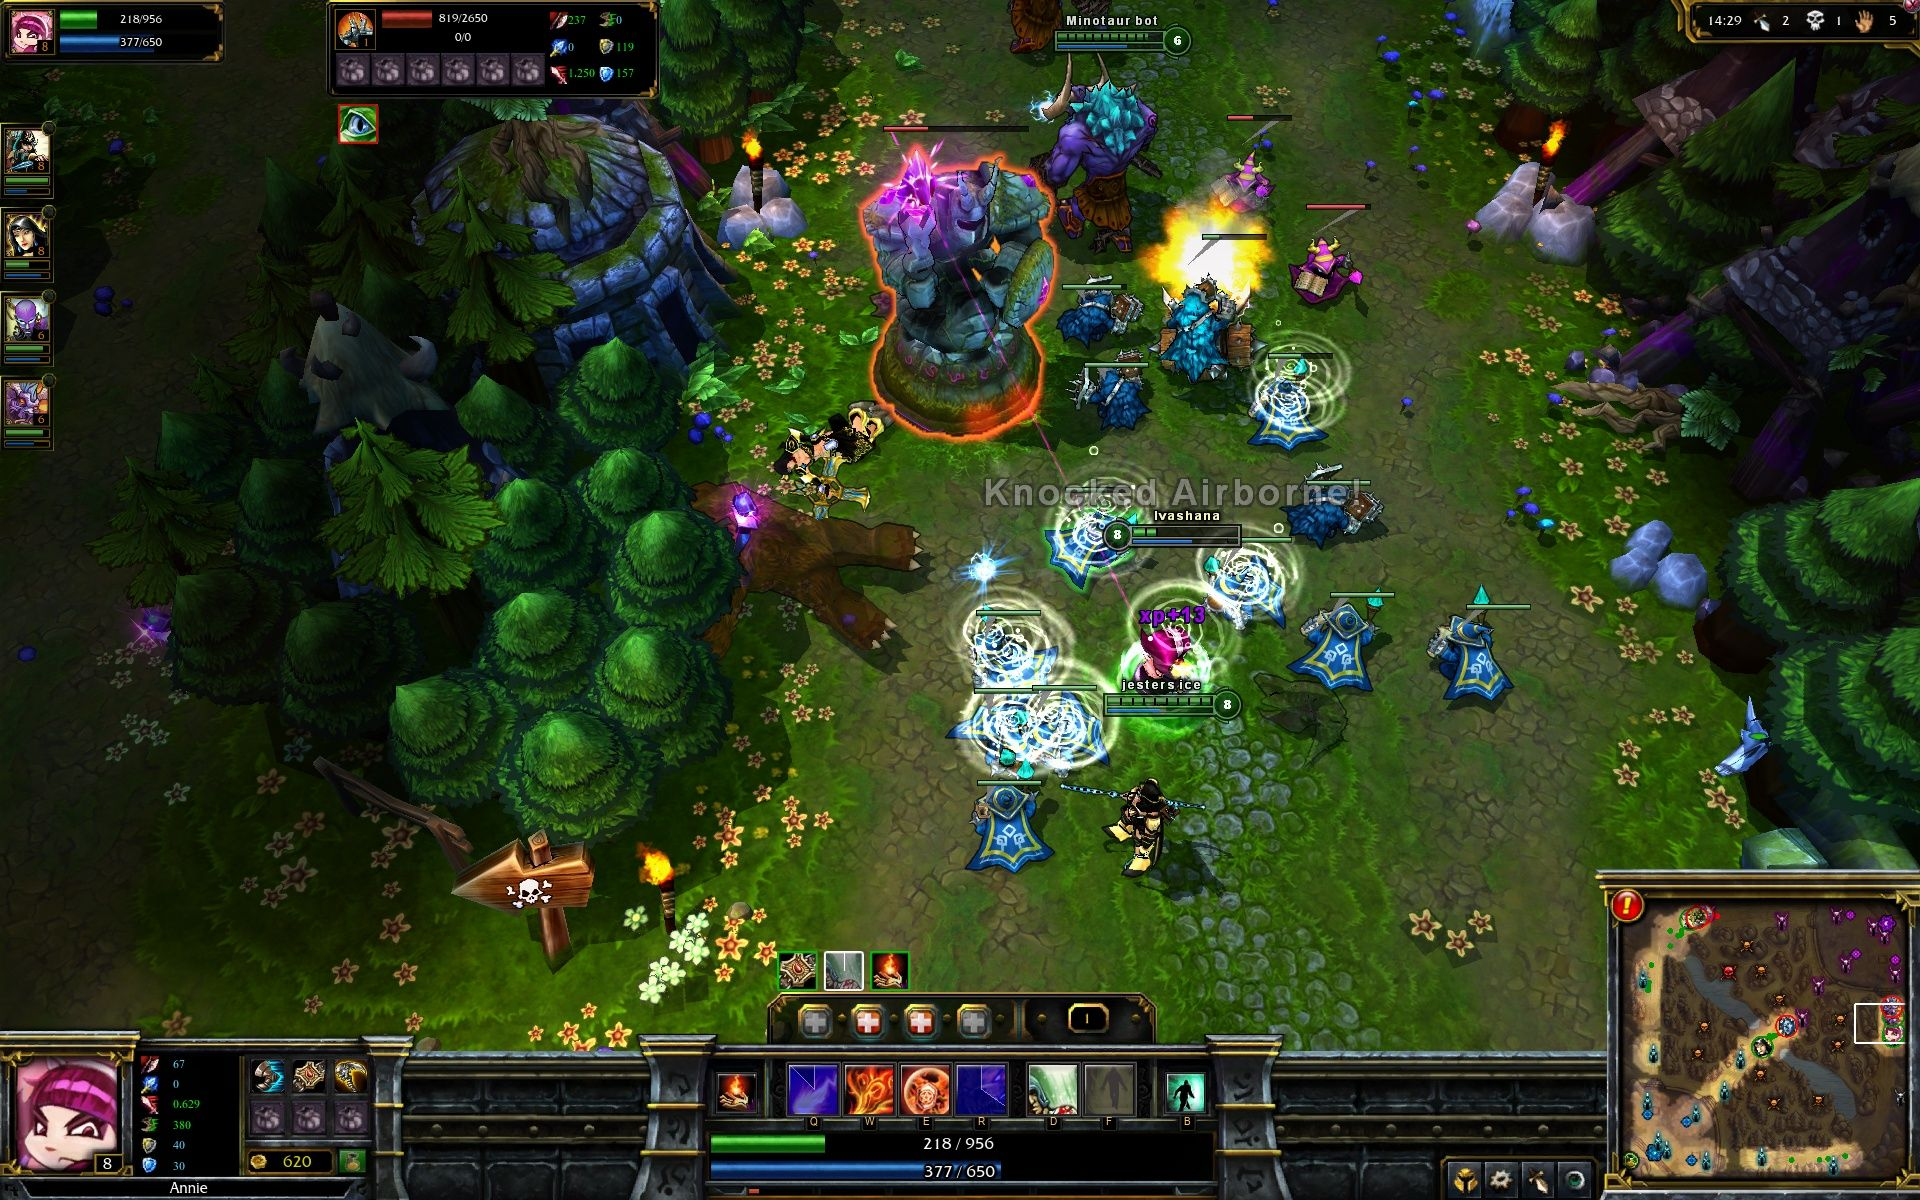
\includegraphics[width=0.8\textwidth]{images/estadodelarte/mercado/foto-lol}
    \caption{\citegame{league_of_legends}, uno de los eSports más populares}
\end{figure}

Para una empresa pequeña, la producción de un eSports es, en principio, inabarcable. Esto se debe principalmente la elevada inversión mencionada anteriormente. Sin embargo, la asociación con unos los partners correctos, ya establecidos en el sector, que pudieran invertir en el producto y le den visibilidad, puede dar una gran oportunidad a los pequeños desarrolladores que cuentan con una mayor flexibilidad con respecto a las grandes compañías, lo que les permite adaptarse más rápidamente a un mercado tan cambiante y mantener una relación directa con el feedback del usuario.

\subsubsection{Realidad Virtual y Realidad Aumentada}
La realidad virtual (normalmente abreviada como VR por las siglas inglesas de Virtual Reality) es la tecnología generada por sistemas informáticos que proporcionan un entorno audiovisual en 3D el que el usuario puede experimentar una inmersión total. Para ello, se hacen usos de cascos especiales equipados con pantallas y sensores de movimiento, los cuales normalmente se complementan con mandos equipados también con sensores para permitir una interacción más natural.
Por otro lado, la Realidad Aumentada o AR es una tecnología que superpone una capa de gráficos generados por ordenador sobre el entorno que rodea al jugador, con la que este puede interaccionar en tiempo real. A diferencia de la VR, no se requiere obligatoriamente de un hardware especial para poder implementar AR; basta únicamente de un dispositivo equipado con una pantalla y una cámara de vídeo, como podría ser un Smartphone.

\begin{figure}[h]
    \centering
    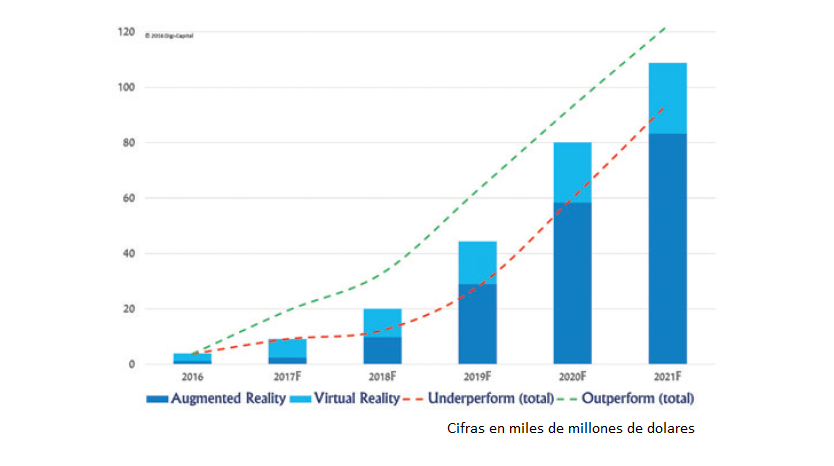
\includegraphics[width=0.8\textwidth]{images/estadodelarte/mercado/crecimiento-vr}
    \caption{Previsiones de crecimiento del mercado de Realidad Virtual y Aumentada
(miles de millones de dólares))}
\end{figure}

Actualmente, existen varias propuestas de diversas compañías en lo que a equipo de VR se refiere. Vamos a mencionar algunas de las más importantes:
\begin{itemize}
\item \textbf{HTC Vive\footnote{https://www.vive.com/}}: es la propuesta de HTC y Valve, orientada a jugadores ``hardcore'' de PC. Disponible desde abril de 2016, el dispositivo requiere de un PC de gama alta (Valve recomienda un PC con una gráfica GeForce GTX 970). El kit de hardware incluye el casco equipado con dos pantallas de 1080x1200 puntos y 90Hz de frecuencia de actualización, dos sensores espaciales y dos mandos para registrar los movimientos de ambas manos, lo que crea le permite crear un entorno 100\% virtual en el que sumergir al jugador.

\item \textbf{OCULUS Rift\footnote{https://www.oculus.com/rift/}}: Es la propuesta más veterana de la lista. Empezó como un exitoso proyecto de Kickstarter en 2012 que más tarde fue adquirida por la empresa Facebook dos años más tarde. Al igual que HTC Vive, Oculus está formado por un casco equipado con pantallas de alta resolución, mandos con sensores de movimiento y dos sensores de posición. El equipo necesita estar conectado a un PC de alta gama para poder funcionar correctamente.

\item \textbf{Samsung Gear VR\footnote{http://www.samsung.com/es/wearables/gear-vr-sm-r325nzvaphe/}}: La propuesta de Samsung es mucho más sencilla y económica, orientado más a la reproducción de vídeo en 360º (concepto similar a la realidad virtual pero con interactividad limitada). El casco incluye una única pantalla y sus mandos carece de detección de movimiento. Estas limitaciones conllevan, por otro lado, un precio mucho más accesible que el de las otras alternativas (99€ contra los más de 500€ de las propuestas más completas)

\item \textbf{SONY PlayStation VR\footnote{https://www.playstation.com/explore/playstation-vr/}}: la propuesta de Sony fue lanzada en el año 2016. Al igual que otras alternativas, el sistema se basa en un casco equipado con dos pantallas y sensores de movimiento, pero su principal punto de venta es su compatibilidad con la consola PlayStation 4 de la misma marca. Esto permite aprovechar la potencia y los mandos de control de está de la consola.
\end{itemize}

\begin{figure}[!htb]
   \begin{minipage}{0.24\textwidth}
     \centering
     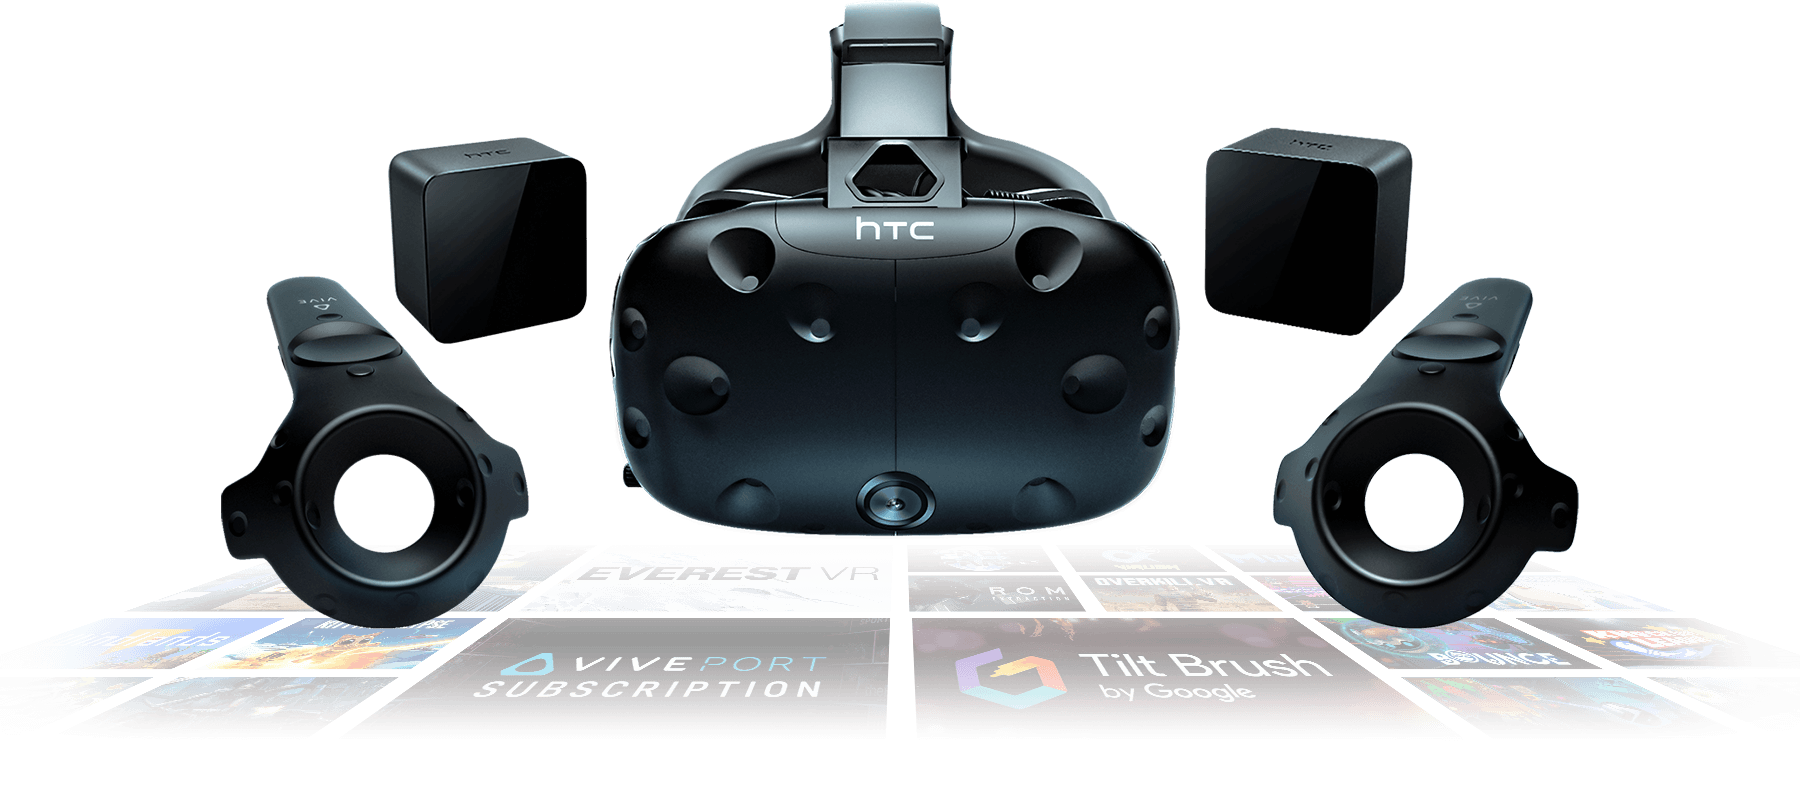
\includegraphics[width=0.7\linewidth, right]{images/estadodelarte/mercado/foto-htc-hive}
   \end{minipage}\hfill
   \begin {minipage}{0.24\textwidth}
     \centering
     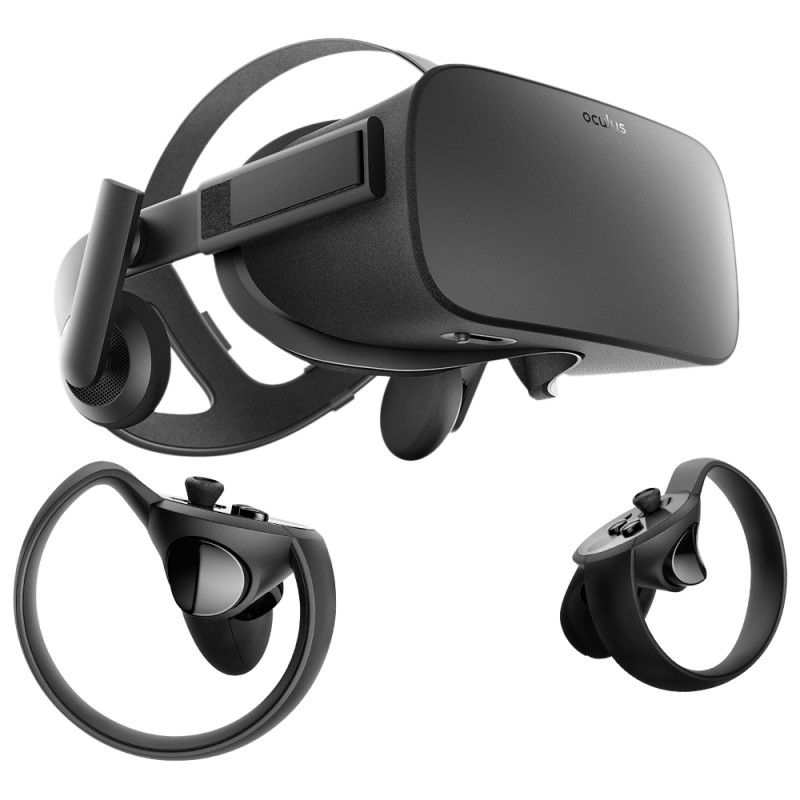
\includegraphics[width=0.7\linewidth, left]{images/estadodelarte/mercado/foto-oculus}
   \end{minipage}
      \begin {minipage}{0.24\textwidth}
     \centering
     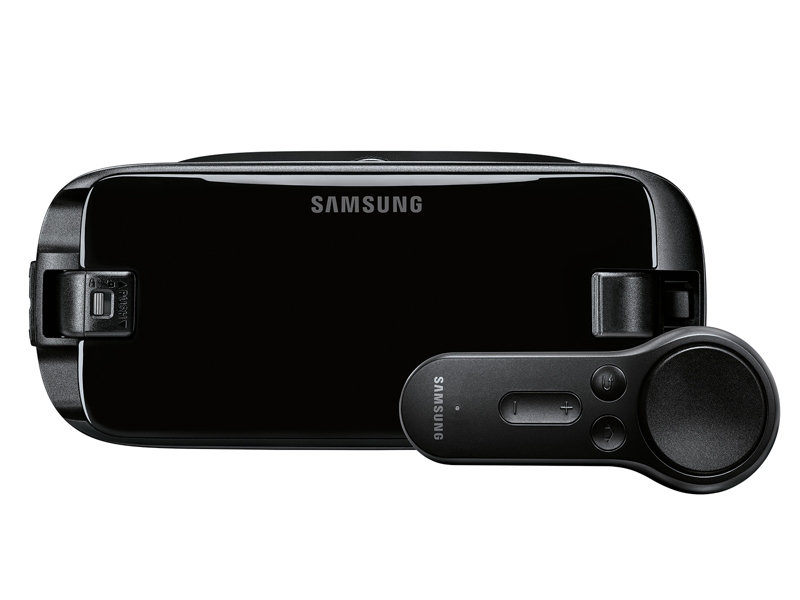
\includegraphics[width=0.7\linewidth, left]{images/estadodelarte/mercado/foto-samsung-vr}
   \end{minipage}
      \begin {minipage}{0.24\textwidth}
     \centering
     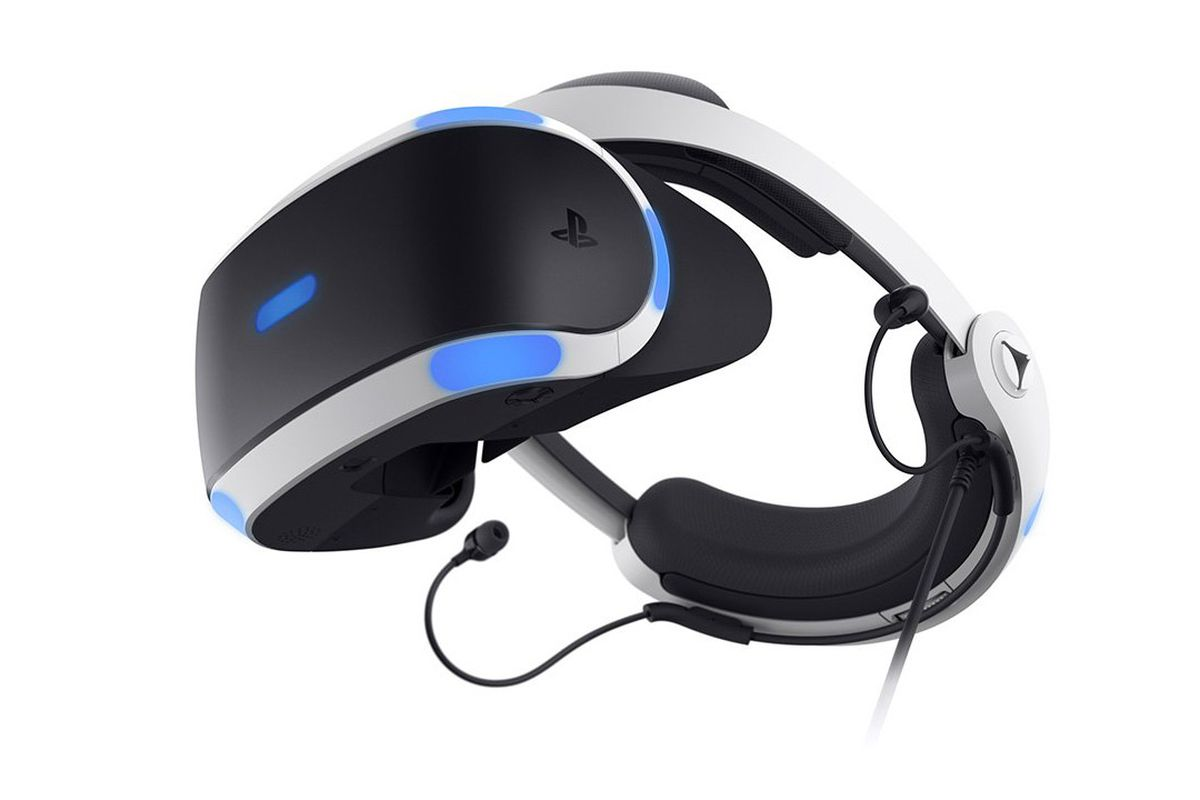
\includegraphics[width=0.7\linewidth, left]{images/estadodelarte/mercado/foto-sony-vr}
   \end{minipage}
   \caption{De izquierda a derecha HTC Vive, Oculus Rift, Samsung VR y PlayStation VR}
\end{figure}

\subsubsection{Web 4.0}
El termino Industria 4.0 fue acuñado por el Ministerio de Educación y Desarrollo alemán en su plan estratégico de 10 puntos del año 2016 para mejorar la educación, investigación e industria del país para adaptarlas a las tecnologías de Internet \cite{web_4_0}. La estrategia trata cinco áreas principales:
\begin{itemize}
\item Fuerte cooperación entre la investigación científica y las empresas.
\item Aumentar la innovación en el sector privado.
\item Diseminar las tecnologías punteras.
\item Internacionalizar la investigación y desarrollo.
\item Fondos para individuos con talento.
\end{itemize}

\begin{figure}[h]
    \centering
    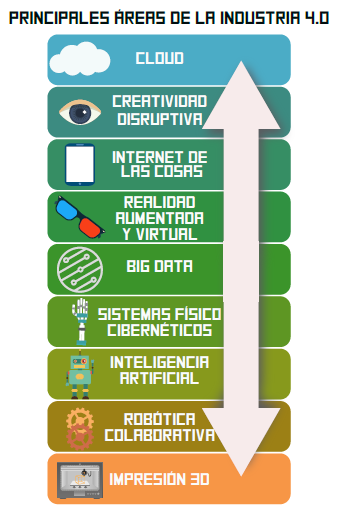
\includegraphics[width=0.6\textwidth]{images/estadodelarte/mercado/tabla-web-4}
    \caption{Áreas de la Industria 4.0}
\end{figure}

De entre las distintas tecnologías que podrían categorizarse como parte de la industria 4.0, vamos a describir aquellas que tienen mayores aplicaciones en el desarrollo de videojuegos:

La computación en la nube, o Cloud Computing, es la tecnología que permite el acceso a servicios informáticos de forma rápida y sencilla a través de Internet. Aunque aún no se a podido implementar correctamente el Cloud Gaming (donde el juego es íntegramente ejecutado en la nueve, reduciendo la exigencia de potencia del sistema del jugador), si se utilizan sistemas en la nube en distintas áreas de los videojuegos. Especialmente notable es su uso para el control y almacenamiento de información en juegos multijugador en línea.

El Internet de las cosas es como se conoce a la tecnología que permite dotar de conexión a Internet a todo tipo de pequeños dispositivos como relojes, sistemas de domótica, drones, sensores de todo tipo, robots, etc. Esto permite implementar videojuegos en todo tipo de sistemas, desde consolas portátiles cada vez más pequeñas y económicas, pasando por juguetes interactivos y llegando a la posibilidad de gamificar con facilidad procesos industriales.

Big Data es el proceso de clasificar grandes volúmenes de datos para poder obtener relaciones interesantes y no evidentes entre ellos. El principal uso de las técnicas de BigData en la industria del Videojuego es el análisis de la información de los jugadores. Analizando datos de los jugadores tales como el género, la edad, la localización geográfica, los intereses, los gastos realizados, etc. es posible obtener estrategias de negocios eficientes.

Los sistemas Ciberfísicos son un nuevo tipo de sistemas con unos componentes hardware y software estrechamente interconectados, cada uno operando en su propio ámbito, operando e interaccionando de forma distinta dependiendo del contexto\cite{cyber_physics}. Entre sus aplicaciones se encuentran las redes eléctricas inteligentes, los sistemas de conducción automática de aviones y automóviles o la monitorización médica. Las interfaces de estos sistemas requieren de unas interfaces con un fuerte ``lado humano'' que permita un uso sencillo e intuitivo. Aquí se podrían utilizar los principios de diseño de juego que permitirían desarrollar un mejor puente entre el lado máquina y la parte de usuario.

La Impresión 3D, también conocida como la producción aditiva es una tecnología que permite producir objetos de forma más sencilla que con las técnicas anteriores. En combinación con las técnicas de escaneado 3D, los estudios de videojuego pueden generar de forma rápida y eficiente modelos 3D de todo tipo (personajes, mapas, objetos...).

\begin{figure}[h]
    \centering
    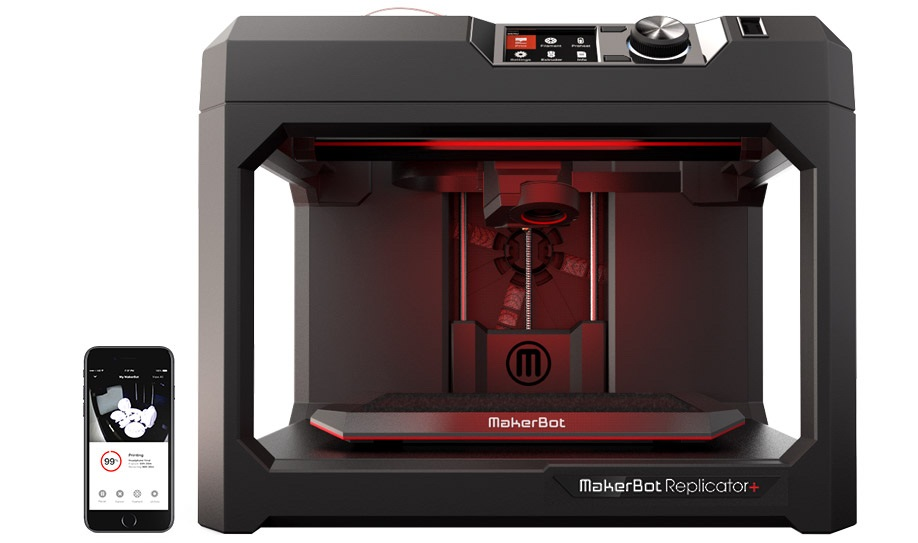
\includegraphics[width=0.8\textwidth]{images/estadodelarte/mercado/impresion-3d}
    \caption{Impresora 3d ``replicator'' de la compañía Makerbot.}
\end{figure}

Las nuevas tecnologías de la industria 4.0 serán de gran ayuda para el desarrollo de videojuego. Pero es posible que la industria 4.0 también ofrezca valor a la industria 4.0 en su conjunto. Dado que la creación de videojuegos es una actividad industrial que está vinculada a diferentes áreas de conocimiento que trabajan juntas para conseguir ofrecer un producto, las técnicas y paradigmas utilizados tienen mucho en común con la nueva forma de trabajar de la industria 4.0, por lo que es posible que puedan extrapolarse a otras industrias, permitiendo una mejor adaptación a los cambios.
